\documentclass[a4paper, 12pt, onecolumn]{article} 

% arara: pdflatex 
% arara: bibtex
% arara: pdflatex
% arara: pdflatex
% arara: clean: {extensions: [ aux, bbl, out, toc, blg, thm ]}

\usepackage[doi, natbibapa]{apacite}

\usepackage{enumitem}
\usepackage[english]{babel}
%if french
%\frenchbsetup{StandardLists=true}

\usepackage[T1]{fontenc}
\usepackage[utf8]{inputenc}

\usepackage{lmodern}

\let\CheckCommand\providecommand
\usepackage{microtype}
\usepackage{hyperref}
%\usepackage[pagebackref=true]{hyperref}
%\renewcommand*{\backrefalt}[4]{#1}

\usepackage{lscape}
\usepackage{graphicx}
\usepackage{amssymb,amsmath}
\usepackage{url}
\usepackage{longtable}
\usepackage{tabu}
\usepackage{siunitx}                        
%\usepackage{threeparttable} 
\usepackage{array}
\usepackage{booktabs}

%\usepackage[french]{authblk}
%\DeclareCaptionFormat{twodot}{:}
\usepackage[font=small,skip=1em]{caption}


\usepackage{setspace}
\usepackage{fullpage}
\usepackage{eso-pic}

\usepackage[explicit, clearempty]{titlesec}
\usepackage[tableposition=top]{caption}
%\usepackage{titlesec}
\usepackage[a4paper]{geometry}

\usepackage{adjustbox}
\usepackage{rotating}
\usepackage{hvfloat}
\usepackage{wrapfig}
\usepackage{tfrupee}  
%\usepackage{multicol}

\usepackage{calc}

\usepackage{lettrine}
\usepackage{oldgerm}

\usepackage{fancyhdr}
\usepackage{lipsum}  
\usepackage{lastpage}

\usepackage{changepage}

% *****************************************************************
% Annexes
% *****************************************************************
%\usepackage[title, titletoc]{appendix}
\usepackage[toc,page]{appendix}
%\renewcommand\appendixtocname{Annexes}
%\renewcommand\appendixname{Annxes}
%\renewcommand\appendixpagename{Annexes}

% *****************************************************************
% Estout related things
% *****************************************************************
\newcommand{\sym}[1]{\rlap{#1}}

\let\estinput=\input% define a new input command so that we can still flatten the document

\newcommand{\estwide}[3]{
		\vspace{.75ex}{
			\begin{tabular*}
			{\textwidth}{@{\hskip\tabcolsep\extracolsep\fill}l*{#2}{#3}}
			\toprule
			\estinput{#1}
			\bottomrule
			\addlinespace[.75ex]
			\end{tabular*}
			}
		}	

\newcommand{\estauto}[3]{
		\vspace{.75ex}{
			\begin{tabular}{l*{#2}{#3}}
			\toprule
			\estinput{#1}
			\bottomrule
			\addlinespace[.75ex]
			\end{tabular}
			}
		}

% Allow line breaks with \\ in specialcells
	\newcommand{\specialcell}[2][c]{%
	\begin{tabular}[#1]{@{}c@{}}#2\end{tabular}}

% *****************************************************************
% Custom subcaptions
% *****************************************************************
% Note/Source/Text after Tables
\newcommand{\figtext}[1]{
	\vspace{-1.9ex}
	\captionsetup{justification=justified,font=footnotesize}
	\caption*{\hspace{6pt}\hangindent=1.5em #1}
	}
\newcommand{\fignote}[1]{\figtext{\emph{Note:~}~#1}}

\newcommand{\figsource}[1]{\figtext{\emph{Source:~}~#1}}

% Add significance note with \starnote
\newcommand{\starnote}{\figtext{* p < 0.1, ** p < 0.05, *** p < 0.01. Standard errors in parentheses.}}

% *****************************************************************
% siunitx
% *****************************************************************
\usepackage{siunitx} % centering in tables
	\sisetup{
		detect-mode,
		tight-spacing		= true,
		group-digits		= false ,
		input-signs		= ,
		input-symbols		= ( ) [ ] - + *,
		input-open-uncertainty	= ,
		input-close-uncertainty	= ,
		table-align-text-post	= false
        }

% *****************************************************************
% Sources
% *****************************************************************
\newcommand{\sourcetab}[1]{\vspace{-1em} \caption*{ \textbf{Source}: {#1}} }
\newcommand{\sourcefig}[1]{\vspace{-2em} \caption*{ \textbf{Source}: {#1}} }

\addto\captionsenglish{\renewcommand{\figurename}{\textbf{Figure}}}
\addto\captionsenglish{\renewcommand{\tablename}{\textbf{Table}}}


% *****************************************************************
% Abstract
% *****************************************************************
\let\abstractname\abstracteng

% *****************************************************************
% Hypothèses
% *****************************************************************
\usepackage{ntheorem}
\theoremseparator{:}
\newtheorem{hyp}{Hypothesis}

% \makeatletter
% \newcounter{subhyp} 
% \let\savedc@hyp\c@hyp
% \newenvironment{subhyp}
 % {%
  % \setcounter{subhyp}{0}%
  % \stepcounter{hyp}%
  % \edef\saved@hyp{\thehyp}% Save the current value of hyp
  % \let\c@hyp\c@subhyp     % Now hyp is subhyp
  % \renewcommand{\thehyp}{\saved@hyp\alph{hyp}}%
 % }
 % {}
% \newcommand{\normhyp}{%
  % \let\c@hyp\savedc@hyp % revert to the old one
  % \renewcommand\thehyp{\arabic{hyp}}%
% } 
% \makeatother

% *****************************************************************
% Tableaux
% *****************************************************************
\addto\captionsfrench{\def\tablename{\textsc{Table}}}

% *****************************************************************
% Bigcenter
% *****************************************************************
%%% ----------debut de bigcenter.sty--------------
 
%%% nouvel environnement bigcenter
%%% pour centrer sur toute la page (sans overfull)
 
%\newskip\@bigflushglue \@bigflushglue = -100pt plus 1fil
 
%\def\bigcenter{\trivlist \bigcentering\item\relax}
%\def\bigcentering{\let\\\@centercr\rightskip\@bigflushglue%
%\leftskip\@bigflushglue
%\parindent\z@\parfillskip\z@skip}
%\def\endbigcenter{\endtrivlist}
 
%%% ----------fin de bigcenter.sty--------------
%%%% fin macro %%%%
\makeatletter
\newskip\@bigflushglue \@bigflushglue = -100pt plus 1fil
\def\bigcenter{\trivlist \bigcentering\item\relax}
\def\bigcentering{\let\\\@centercr\rightskip\@bigflushglue%
\leftskip\@bigflushglue
\parindent\z@\parfillskip\z@skip}
\def\endbigcenter{\endtrivlist}
\makeatother

% *****************************************************************
% Lignes de code
% *****************************************************************
\usepackage{listings}
\lstset{ 
basicstyle=\scriptsize\ttfamily,
breaklines=true,
keywordstyle=\bf \color{blue},
commentstyle=\color[gray]{0.5},
stringstyle=\color{red},
showstringspaces=false,
numbers=left,
numberstyle=\tiny \bf \color{blue},
stepnumber=1,
numbersep=10pt,
firstnumber=1,
numberfirstline=true,
frame=leftline,
xleftmargin=0.5cm
}
 
% *****************************************************************
% Auteurs en bleu
% *****************************************************************
%\renewcommand{\citep}[1]{\textcolor{teal}{\citep{#1}}}
%\renewcommand{\cite}[1]{\textcolor{teal}{\cite{#1}}}
\usepackage{xcolor}
\usepackage{colortbl}

\hypersetup{colorlinks,linkcolor={red},citecolor={teal},urlcolor={blue}}
%\newcommand{\ypenser}[1]{\textcolor[purple]{#1}}
\newcommand{\ypenser}[1]{\textbf{\color{purple}--#1--}}

% *****************************************************************
% Mail
% *****************************************************************
\newcommand{\email}[1]{\href{mailto:#1}{\nolinkurl{#1}}}

% *****************************************************************
% Résumé et mots clés
% *****************************************************************
 \newenvironment{resab}[1]
{\begin{adjustwidth}{0cm}{0cm} \hangafter =1\par
    {\normalsize\bfseries #1\ \\ }\normalsize}
{\end{adjustwidth}\medskip}

 \newenvironment{keywords}
{\begin{adjustwidth}{0cm}{0cm} \hangafter =1\par
    {\normalsize\itshape Keywords:}~\normalsize}
{\end{adjustwidth}\medskip}

 \newenvironment{jelcodes}
{\begin{adjustwidth}{0cm}{0cm} \hangafter =1\par
    {\normalsize\itshape JEL Codes:}~\normalsize}
{\end{adjustwidth}\medskip}

% *****************************************************************
% Poete
% *****************************************************************
\newcommand{\attrib}[1]{%
\nopagebreak{\raggedleft\footnotesize #1\par}}

% *****************************************************************
% Stata
% *****************************************************************
\newcommand{\Stata}{%
\textsc{Stata$^{\mbox{\scriptsize{\textregistered}}}$}
}

% *****************************************************************
% Encadré
% *****************************************************************
\usepackage{tikz}

% Thick
\def\checkmark{\tikz\fill[scale=0.4](0,.35) -- (.25,0) -- (1,.7) -- (.25,.15) -- cycle;} 

\newcommand{\titlebox}[2]{%
\tikzstyle{titlebox}=[rectangle,inner sep=10pt,inner ysep=10pt,draw]%
\tikzstyle{title}=[fill=white]%
%
\bigskip\noindent\begin{tikzpicture}
\node[titlebox] (box){%
    \begin{minipage}{0.94\textwidth}
#2
    \end{minipage}
};
%\draw (box.north west)--(box.north east);
\node[title] at (box.north) {#1};
\end{tikzpicture}\bigskip%
}

% *****************************************************************
% Changer la forme des titres
% *****************************************************************
 %\titleformat{\section}[block]			%section + style prédéfini par l'extension (block = 1 ligne)
 %{\sffamily\bfseries\LARGE\titlerule[1pt]}						%format pour le titre + label
 %{\sffamily\bfseries\LARGE}						%format pour le titre + label
 %{\sffamily\bfseries\LARGE\arabic{section}}		%format que pour le label
 %{0.5cm}								%espace qui sépare le label du titre
 %{#1}									%description du style pour le titre uniquement
 %\titlespacing{\section}				%section
 %{0cm}									%espace à gauche du titre
 %{3em}									%espace verticale AVANT le titre
 %{1em}									%espace verticale APRES le titre
 %%{0cm} 								%espace à droite du titre: mettre la même valeur que gauche pour un peu centrer

 %\titleformat{\subsection}{\sffamily\bfseries\Large}{\thesubsection}{0.4cm}{#1}
 %\titlespacing{\subsection}
 %{1cm}
 %{2em}
 %{1ex}

 %\titleformat{\subsubsection}{\sffamily\bfseries\large}{\thesubsubsection}{0.4cm}{#1}
 %\titlespacing{\subsubsection}
 %{2cm}
 %{2em}
 %{1ex}

% *****************************************************************
% Style de la date
% *****************************************************************
%\def\mydate{\leavevmode\hbox{\the\year-\twodigits\month}}
\def\mydate{\leavevmode\hbox{\the\month-\twodigits\year}}
\def\twodigits#1{\ifnum#1<10 0\fi\the#1}

% *****************************************************************
% En tête
% *****************************************************************

% Pour les numéros de pages
%\pagestyle{fancy}

% Si tu veux mettre les numéros genre: 1/22
% Il faut que tu écrives
% "\thepage/\pageref{LastPage}"
% Sans les " " dans les lignes en bas: \fancyhead[...

% Ca c'est pour enlever la barre horizontale sous l'entête
% Pour la laisser tu mets "1pt" au lieu de 0
\renewcommand{\headrulewidth}{0pt}
\renewcommand{\footrulewidth}{0pt}

% fancyhead pour l'entête
% fancyfoot pour le pied de page
% L=left; R=right; C=center
%\fancyhead[L]{\textcolor{gray}{\textsf{\textit{Revue de la littérature autour du mariage: le cas de l'Inde}}}}
%\fancyhead[R]{\textcolor{gray}{\textsf{Natal, A. (\mydate)}}}
%\fancyfoot[C]{\thepage}
%updmap.exe --admin

%\lhead{\textcolor{gray}{\textsf{\textit{Revue de la littérature autour du mariage: le cas de l'Inde}}}}
%\rhead{\textcolor{gray}{\textsf{Natal, A. (\mydate)}}}
\cfoot{\thepage}

% *****************************************************************
% Jatis
% *****************************************************************
\newcommand{\jati}[1]{\textit{j\={a}ti{#1}}}

% *****************************************************************
% Enlever le titre Table des matières
% *****************************************************************
%\makeatletter
%\renewcommand\tableofcontents{%
%    \@starttoc{toc}%
%}
%\makeatother

% *****************************************************************
% À développer
% *****************************************************************
\newcommand\dev[1]{\textbf{\textcolor{red}{#1}}}

% *****************************************************************
% Fonts
% *****************************************************************
%\usepackage{tgbonum}
\usepackage{kpfonts}

% *****************************************************************
% Taille des tableaux
% *****************************************************************
\let\oldtabular=\tabular
\def\tabular{\small\oldtabular}
%\def\tabular{\normalsize\oldtabular}

% *****************************************************************
% Style de la biblio
% *****************************************************************
\bibliographystyle{apacite}

% *****************************************************************
% Numérotation
% *****************************************************************
%\usepackage{lineno}

% *****************************************************************
% Titre et page de garde
% *****************************************************************
\usepackage{titling}
\setlength{\droptitle}{-2cm}
\pretitle{\begin{center}\fontsize{24pt}{10pt}\selectfont\bfseries}
\posttitle{\par\end{center}\vskip 1ex}
\preauthor{\begin{center}
    \large \lineskip 0.5em}
\postauthor{\par\end{center}}
%\thanksheadextra{1,}{}
\thanksheadextra{}{}
\setlength\thanksmarkwidth{.5em}
\setlength\thanksmargin{-\thanksmarkwidth}


% *****************************************************************
% Symboles
% *****************************************************************

\def\@fnsymbol#1{\ensuremath{\ifcase#1\or *\or \dagger\or \ddagger\or
   \mathsection\or \mathparagraph\or \|\or **\or \dagger\dagger
   \or \ddagger\ddagger \else\@ctrerr\fi}}
   
\makeatletter
\newcommand{\ssymbol}[1]{^{\@fnsymbol{#1}}}
\makeatother
   
   
   
% *****************************************************************
% Makecell
% *****************************************************************
\usepackage{makecell}
\newcommand\Tablenote[2]{\multicolumn{#1}{l}{\makecell[l]{\textit{Note:}~#2}}}


   

%\usepackage{fonttable}

\usepackage{import}

\usepackage[
singlelinecheck=false % <-- important
]{caption}

\usepackage{upgreek}

\newcommand{\ie}{i.e.}
\newcommand{\sd}{standard deviation}
\newcommand{\pp}{percentage points}
\newcommand{\aebe}{all else being equal}
\newcommand{\Aebe}{All else being equal}
\newcommand{\ote}{other things equal}
\newcommand{\Ote}{Other things equal}
\newcommand{\cl}{confidence level}
\newcommand{\lit}{\dev{literature}}
\newcommand{\PTCS}{PT\&CS}





% \renewcommand*\thetable{\Alph{section}.\arabic{table}}
% \renewcommand*\thefigure{\Alph{section}.\arabic{figure}}


% *****************************************************************
% Interlignes et marges
% *****************************************************************
\setstretch{1.5}
\geometry{%
left=2.5cm,
right=2.5cm,
top=2.5cm,
bottom=2.5cm,
%includefoot,
%headsep=1cm,
%footskip=1cm
}%

% *****************************************************************
% Page de garde
% *****************************************************************
\title{Stability of Personality Traits over Time: The case of Rural India}
\author{Arnaud Natal\thanks{Univ. Bordeaux, CNRS, GREThA, UMR 5113, F-33600 \textsc{Pessac, France} - \email{arnaud.natal@u-bordeaux.fr}} ~ \& Christophe J. Nordman\thanks{IRD, UMR LEDa-DIAL, IFP - \email{nordman@dial.prd}} }
\date{\today}
\renewcommand\maketitlehookc{%
  \begin{center}
    %\textsuperscript{1}{\small Université de Bordeaux}
    \textsuperscript{}{\normalsize Very preliminary draft}
  \end{center}}

% ******************************************************************
\begin{document}
\maketitle

\hrule 
\vspace{0.3cm}

\begin{resab}{Abstract}
L'internal consistency est excellente pour 2016-17 et moyenne pour 2020-21.
Cependant, à vérifier en lancant de nouveau les lignes

Cependant, lorsqu'on lance une analyse factorielle pour 2016-17 et une pour 2020-21, on voit que les mêmes facteurs ressortent à peu près et ils sont relativement proche du Big-5, suggérant que ca fonctionne bien


\end{resab}

\begin{keywords}
Gender, caste, panel data, Tamil Nadu.
\end{keywords}

\begin{jelcodes}
\end{jelcodes}

\hrule
%\linenumbers

\clearpage
\newpage
% ******************************
\section{Introduction}
% \addcontentsline{toc}{section}{Introduction}
\label{Introduction}
% ******************************

\begin{itemize}
\item Faire analyse factorielle 2016
\item Faire analyse factorielle 2020
\item Faire FA par sexe, caste et age
\item Organiser le papier
\item Selon moi, si l'objectif c'est de regarder la stabilité, il faut partir de la mesure du Big-5
\item Puis balancer les omega pour montrer la cohérence interne: si élevée alors ca veut dire que le Big-5 est pas dég
\item Aborder la question du biais avec les mesures
\item Montrer que le modèle n'est pas forcément dégueu en 2016 car FA similaire à Big5
\item Pb pour 2020, la FA ne colle pas 
\end{itemize}


Since more than a decade, there has been increasing interest in psychology in economics literature, especially through personality traits and cognitive skills (\PTCS).
The relevance of such analysis in economics is well documented.
\cite{Hanushek2008} show that cognitive skills are correlated with individual earnings, distribution of income and economic growth (and other factors such as well-functioning economic institutions --although enter into growth and may well have stronger effects, may also amplify the effects of cognitive skills).
% Authors add that the current situation in developing countries is much worse than generally pictured on the basis just of school enrolment and attainment.
Regarding personality traits, \cite{Borghans2008} examine, for instance, the relevance of this in economics.
They show that psychological variables are a good predictor of socioeconomic success and especially on the labour market\footnote{For further details see \cite{Almlund2011}.}. %\dev{and they can be influenced by interventions and investment more readily than IQ after the early years because of the non-stability through life cycle.}
Institutions, such as World Bank, collect more and more data\footnote{As stated by \cite{Laajaj2019b}, the World Bank alone spent 1 billion USD a year for data on \PTCS.} on \PTCS~ because it enables a better understanding of skill requirements in the labour market, backward linkages between skills acquisitions and educational achievement, personality, and social background, and forward linkages between skills acquisitions and living standards, reductions in inequality and poverty, social inclusion, and economic growth \citep{STEP2014}.



\paragraph{Definition}
Used in similar studies, personality traits and cognitive skills measure two distinct skills.
Cognitive skills represent the mental processes involved in the acquisition of knowledge, manipulation of information, and reasoning that include the domains of perception, memory, learning, attention, decision-making, and language abilities \citep{Kiely2014} while personality is the dynamic organisation within the individual of those psychophysical systems that determine his characteristic behaviour and thought \citep{Allport1961}.
The Big-5 model constitutes the main personality trait taxonomy\footnote{Among the theories of personality, the traits can be defined as thought, emotion and habitual patterns of behaviour \citep{Kassin2003}.}.
%Based on \cite{Goldberg1981} and \cite{McCrae1987} works, it 
It identifies five dimensions of personality: emotional stability --ES-- (capacity to experience negative emotions); extraversion --EX-- (capacity to experience positive emotions, the tendency to seek stimulation and company from others); openness to experience --OP-- (capacity to be creative and unstructured); agreeableness --AG-- (perceptions of others that are caring, compassionate, and altruistic); conscientiousness --CO-- (capacity to display self-discipline, act dutifully, and strive for achievement against measures or outside expectations).	



\paragraph{Exogeneity of personality traits and cognitive skills}
The exogeneity of \PTCS~ is well assumed because of stability over time while there is no consensus in psychology \citep{Ardelt2000, Deary2014}.

For personality traits, according to \cite{Costa1997, McCrae2000} it remains stable, in part, because it is a genetic predisposition that, by definition, cannot be changed over life.
%\footnote{But not all, see \cite{Borghans2008, Almlund2011, Heckman2011}. As stated by \cite{Heckman2011}, ``Personality traits are not set in stone. They change over the life cycle. They are a possible avenue for intervention and policy.''}
Many economists follow this path and the majority of then assume stability over time after the age of 25 \citep{CobbClark2012} and other verify this stability \citep{CobbClark2011}.
However, the stability refutes sociological and psychological literature which interesting in the influence of childhood and adulthood socialisation on personality \citep{Mortimer1978, Moen1995}.
\cite{Ardelt2000} state that ``personality can change over the course of a person's life, particularly if age at first measurement is low or over 50, if the retest interval is large, if individual personality aspects rather than the overall personality are considered [...].''
However, analysis of stability do not provide sufficient information on change in the social environment and \cite{Ardelt2000} suggests to analyse personality before and after ``unexpected, drastic changes in people's social environments''.
Indeed, such changes can imply a change in the individual personality to adapt to the new environment that they did not select.

Big-5 taxonomy not universal \cite{Gurven2013}


\clearpage
\newpage
% ******************************
\section{Data}
\label{section:data}
% ******************************

Our empirical analysis is based on NEEMSIS-1 \& NEEMSIS-2 (Networks, Employment, dEbt, Mobilities and Skills in India Survey) surveys carried out respectively in 2016-17, and 2020-21 \citep{NEEMSISreport, NEEMSIS2017}.
These surveys are the second and third waves of a longitudinal data collection project\footnote{Project took place within two broader research programmes located within the Observatory of Rural Dynamics and Inequalities (\url{https://odriis.hypotheses.org/}) at the French Institute of Pondicherry, India.} start in 2010 with RUME (RUral Microfinance and Employment survey) project in ten villages of Tamil Nadu.
Located in the Cuddalore and Villupuram districts, a mostly agricultural area, economies benefits from the proximity of two large industrial towns (Neyveli and Cuddalore) and a regional business center (Panruti).

RUME randomly selected 405 households using stratified sample framework based on three dimensions: proximity to small towns (Panruti, Villupuram and Cuddalore), an agro-ecological criterion, and caste affiliation.
Thus, half of villages have irrigated land (the other half is dry) and within villages, half of the sample was selected from the mostly upper and middle caste part of the village (Ur) while the other half from the Colony part, where dalits (the ex-untouchables) mainly live. 
NEEMSIS-1 recovered 388 households (4.19\% attrition rate) and randomly selected 104 news households (for a total of 492 households) from these 10 villages, based on the same method. 
%Given that some households had migrated elsewhere between the 2010 and 2016-17 sampling periods (13\% of the recovered households).
NEEMSIS-2 recovered 485 households (1.42\% attrition rate) from 2016-17 and recovered 10 households from 2010 that were not recovered in 2016-17.
Moreover, 100 news households were randomly selected (for a total of 595 households).

In NEEMSIS-1 \& NEEMSIS-2, two household members, called ``ego 1'' (mostly household questionnaire respondent) and ``ego 2'' (one younger household member randomly selected on a criterion of age), are directly addressed individual questionnaires that provide for instance a range of information on \PTCS.

Regarding the reliability, the great expertise of the team\footnote{Some members of the research team are present since more than 20 years on the region for numerous quantitative and qualitative surveys.} helped to formulate questions appropriately.
Moreover, the moderate magnitude of the survey, compared to nationally representative datasets, ensures the high quality of the data and the tablet-based mode of data collection improved data quality in including constraints on answers to prevent inconsistencies. 


\clearpage
\newpage
% ******************************
\section{Methodology}
% ******************************

	% ******************************
	\subsection{Construction of personality traits \& cognitive skills variables }
	% ******************************

As stated earlier, our survey allows us to construct measures of cognitive skills.
It includes three score variables based on literacy test, numeracy test and Raven progressive matrices test\footnote{Raven matrix is ``a nonverbal test of mental ability consisting of abstract designs, each of which is missing one part. The participant chooses the missing component from several alternatives to complete each design.'' -- \url{https://dictionary.apa.org/ravens-progressive-matrices}. Accessed January 27, 2021.}.
These scores are constructed in adding up the correct answers of a set of four questions for literacy and numeracy test (six for numeracy in 2020-21) and 36 for Raven.
Then, we standardise the score to ensure comparability of results between personality traits and cognitive skills.

Regarding personality traits, on the basis of 35 questions referring to Big-5 taxonomy, we averaged answers --based on a Likert scale from 1-``Almost Never'' to 5-``Almost always'', that belong to a determined trait after correcting for acquiescence bias\footnote{Acquiescence bias represents the tendency to answer more in one direction (agree or disagree) over the other.} (see Appendix \ref{section:efa_big5}).
The resulting mean represents the score on each trait.



	% ******************************
	\subsection{Factor analysis}
	% ******************************

As warned by \cite{Laajaj2019}, the Big-5 taxonomy is limited in developing countries for several reasons: the enumerator-respondent interactions in face-to-face survey can induce a bias; the low education levels can make questions more difficult to understand and can induce a systematic response patterns, especially the acquiescence bias.
The very good knowledge of the field (see section \ref{subsection:data}) allow us to collect data of high quality and avoid a bias due to misunderstanding of questions.
Moreover, we implement our own factor analysis of the 35 questions by principal component with promax rotation.
To avoid a bias in factor analysis, we do not recode reverse questions because it might force likeness with Big-5 taxonomy.
In our dataset, acquiescence bias is measure with a set of reverse questions that are supposed perfectly opposed to another set of questions. 
However, the assumption of opposition is supportable only in the Big-5 taxonomy.
In another layout, pairs of questions can measure different aspects of personality\footnote{\cite{Singh2013} show that in Hindi, the major language spoken in India, three traits different from Big-5 taxonomy firmly stood out.}.
The resulting factors for 2016-17 data are relatively similar to the Big-5 personality traits with satisfactory \citeauthor{McDonald1999}'s $\Upomega$: Factor 1 as Openness-Extraversion ($\Upomega=0.91$); Factor 2 as Conscientiousness ($\Upomega=0.88$); Factor 3 as \textit{Porupillatavan} --Tamil terms for talkative, easily distracted individual-- ($\Upomega=0.69$); Factor 4 as Emotional stability ($\Upomega=0.78$) and Factor 5 as Agreeableness ($\Upomega=0.62$) (see Appendix \ref{section:efa_big5}) while resulting factors for 2020-21 data are very different to the Big-5 taxonomy and to the 2016-17 factors.
We do not present results here because we do not use it as personality traits measure (see section \ref{subsection:econometricframework}), however it is available on request.



\clearpage
\newpage
% ******************************
\section{Results}
% ******************************

Our results show stability for minor part of the population (see Appendix \ref{section:stab_big5}).
Non-corrected traits, in addition to having globally (2016-17 and 2020-21) higher internal consistency (see Table \ref{fig:omega}) are less unstable over time without being able to relate stability.
Evolution of personality traits can be explained by the fact that NEEMSIS-2 data were collected after the first lockdown\footnote{See \url{https://thewire.in/covid-19-india-timeline} for complete timeline of COVID-19 pandemy in India. Accessed August 16, 2021.} (end of 2020) and the associated mental health consequences \citep{Golechha2020, Kochhar2020} can have cause --or at least exacerbated, the non-stability.

Concerning cognitive skills, majority of individuals have higher or equal score in 2020-21 than in 2016-17 (see Appendix \ref{section:stab_big5}) which is consistent with the lifelong learning theory --the continuing development of knowledge and skills that people experience after formal education and throughout their lives \citep{London2011}.


	% ******************************
	\subsection{Acquiescence bias}
	% ******************************
I have calculated acquiescence bias (AB) for all egos of 2016-17 (n=953) and 2020-21 (n=1,316).
Around 0.5, the bias is medium (not too high but not 0), from 1, the bias is too high.
\dev{Le biais se mesure en faisant la moyenne des questions inversées. Les réponses allant de 1 à 5 (1-Almost always; 2-Quite often; 3-Sometimes; 4-Rarely; 5-Almost never), la moyenne obtenue pour un individu sans biais est de 3 (Sometimes) car il est censé répondre aux deux questions (dont une inversée) :
Deux fois Sometimes ou une fois Almost always et une fois Almost never ou une fois Quite often et une fois Rarely. 
Un biais de 0.5 correspond à la combinaison d'1 modalité moins parfaite. Par exemple Almost always et Rarely. Un biais de 1 correspond à une combinaison moins parfaite de 2 modalités. Par exemple Almost always et Sometimes. Un biais supérieur à 1 correspond à une combinaison moins parfaite de 3 ou 4 modalités.}



Figure \ref{fig:ars} shows the distribution of the acquiescence bias in 2016-17 and in 2020-21.
Even if a small part of our population have a high AB, the 2020-21 distribution is more spread out to the right in 2020-21 than in 2016-17, suggesting higher bias.
Intuition is confirmed with Figure \ref{fig:curvears} that shows cumulative distribution of acquiescence bias. 
The flatter the curve is, the lower the acquiescence bias is.
In 2016-17, 50\% of individuals have a bias lower than 0.3 while it is 0.5 in 2020-21.

Figure \ref{fig:arssub} shows that female have higher bias than male. 
In 2020-21, by caste, 


	% ******************************
	\subsection{Internal consistency}
	% ******************************

\citeauthor{McDonald1999}'s $\Upomega$\footnote{Literature on internal consistency estimators increasingly agrees that \citeauthor{Cronbach1951}'s $\upalpha$ --the widest used estimator is maybe not very efficient \citep{Bourque2019, TrizanoHermosilla2016}.}, a measure of internal consistency, are mostly satisfactory for 2016-17 data corrected from acquiescence bias: 0.81 for openness; 0.86 for conscientiousness; 0.59 for extraversion; 0.60 for agreeableness and 0.80 for emotional stability (see Figure \ref{fig:omega}).
For 2020-21, the internal validity after correcting for acquiescence bias is not ideal compared to non-corrected items.
It implies that results could suffer from measurement error, which would bias our results towards zero.



	% ******************************
	\subsection{Factor analysis}
	% ******************************






\clearpage
\newpage
\section{Corrected items}

\begin{figure}[!h]
\raggedright
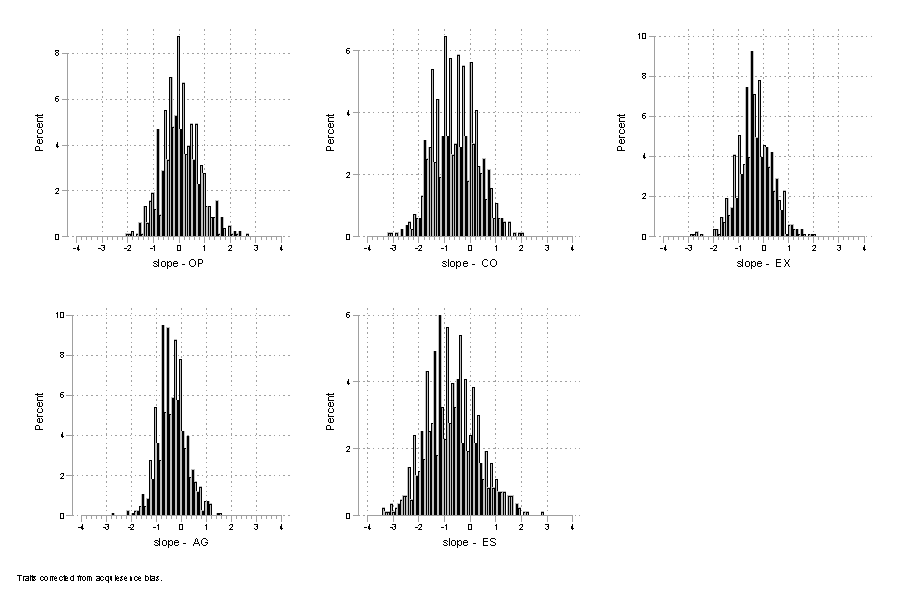
\includegraphics[scale=0.8]{INPUT/diffcont_cor}
\caption{}
\sourcefig{NEEMSIS-1 (2016-17) \& NEEMSIS-2 (2020-21); author's calculations.}
\label{fig:diffagecor}
\end{figure}

\begin{figure}[!h]
\raggedright
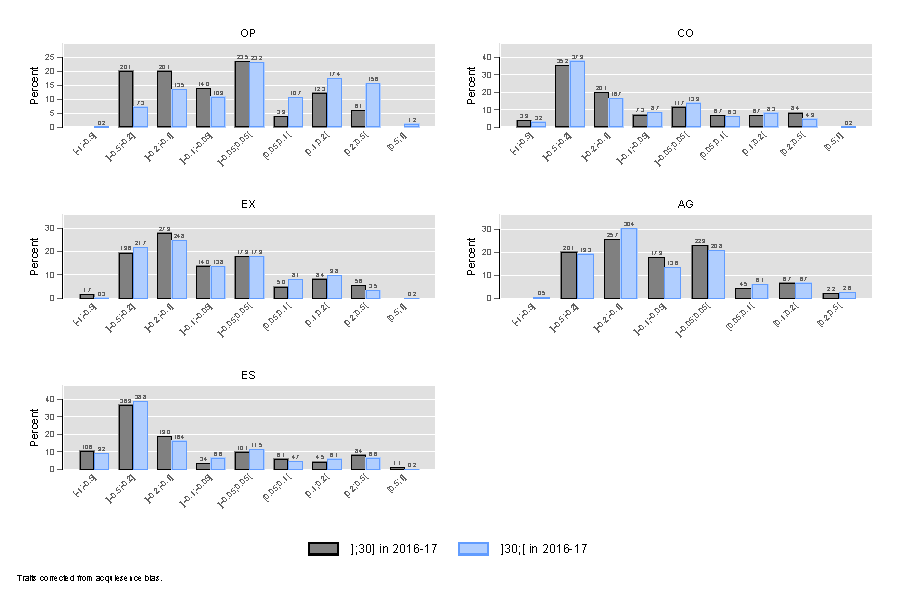
\includegraphics[scale=0.8]{INPUT/diff_age_cor}
\caption{}
\sourcefig{NEEMSIS-1 (2016-17) \& NEEMSIS-2 (2020-21); author's calculations.}
\label{fig:diffagecor}
\end{figure}

\begin{figure}[!h]
\raggedright
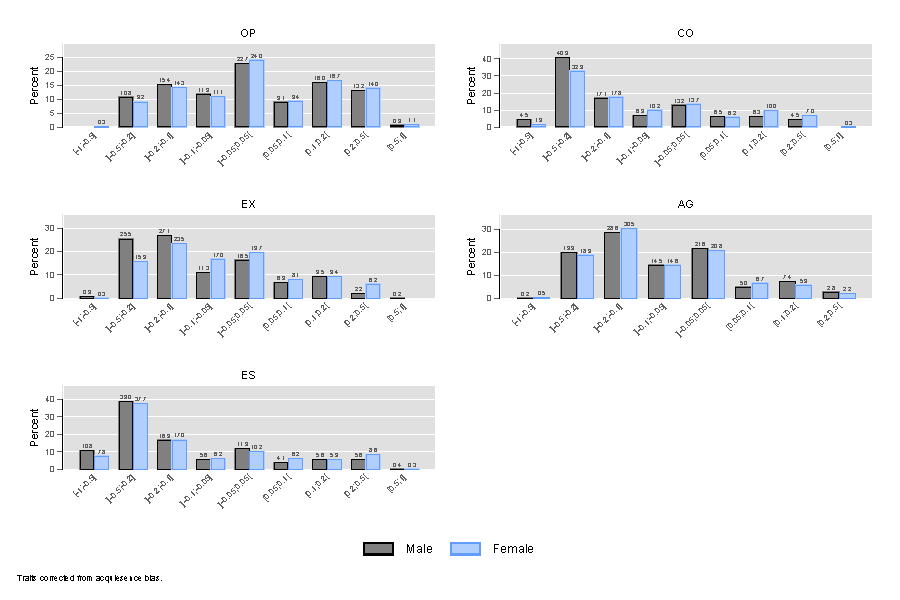
\includegraphics[scale=0.8]{INPUT/diff_gender_cor}
\caption{}
\sourcefig{NEEMSIS-1 (2016-17) \& NEEMSIS-2 (2020-21); author's calculations.}
\label{fig:diffgendercor}
\end{figure}

\begin{figure}[!h]
\raggedright
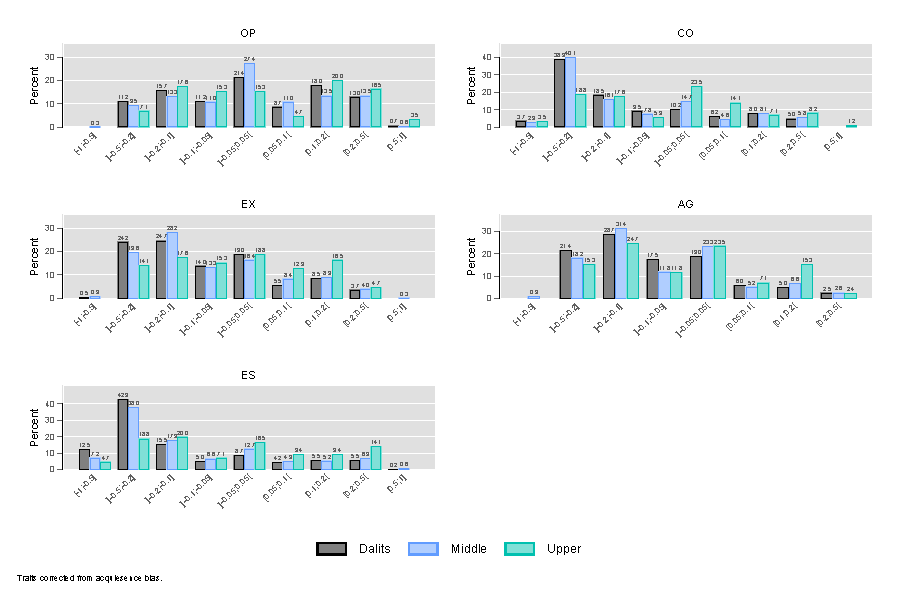
\includegraphics[scale=0.8]{INPUT/diff_caste_cor}
\caption{}
\sourcefig{NEEMSIS-1 (2016-17) \& NEEMSIS-2 (2020-21); author's calculations.}
\label{fig:diffcastecor}
\end{figure}



\clearpage
\newpage
\section{Non-corrected items}

\begin{figure}[!h]
\raggedright
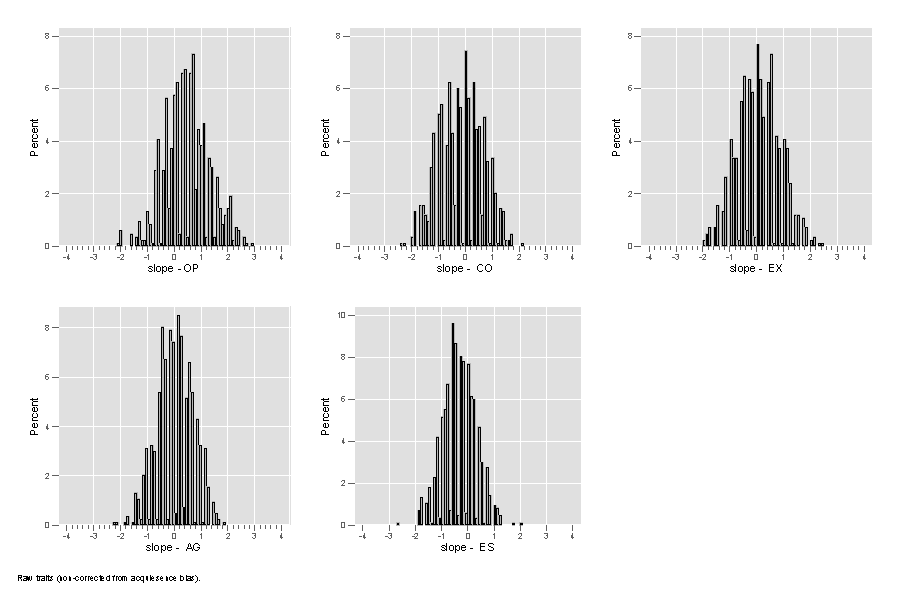
\includegraphics[scale=0.8]{INPUT/diffcont_raw}
\caption{}
\sourcefig{NEEMSIS-1 (2016-17) \& NEEMSIS-2 (2020-21); author's calculations.}
\label{fig:diffagecor}
\end{figure}

\begin{figure}[!h]
\raggedright
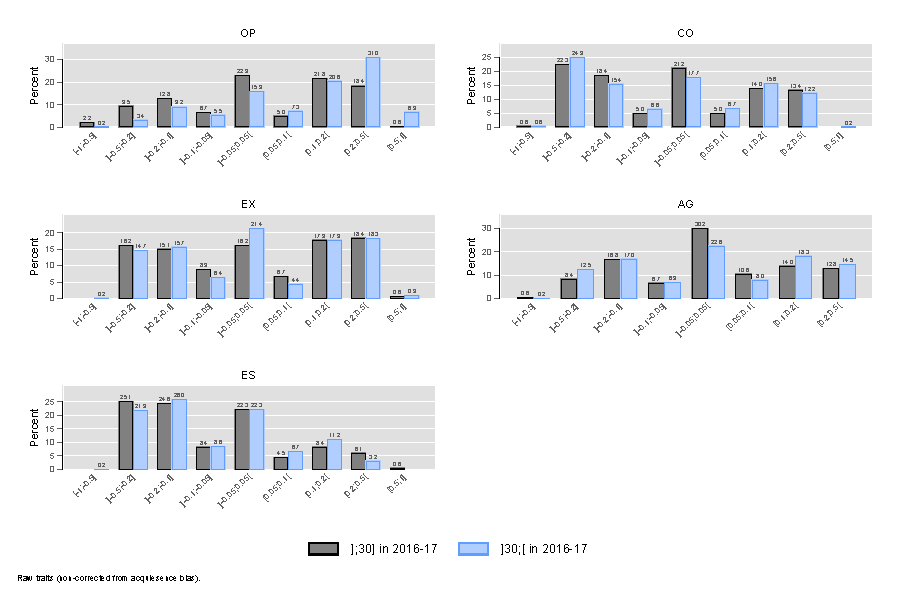
\includegraphics[scale=0.8]{INPUT/diff_age_raw}
\caption{}
\sourcefig{NEEMSIS-1 (2016-17) \& NEEMSIS-2 (2020-21); author's calculations.}
\label{fig:diffagecor}
\end{figure}

\begin{figure}[!h]
\raggedright
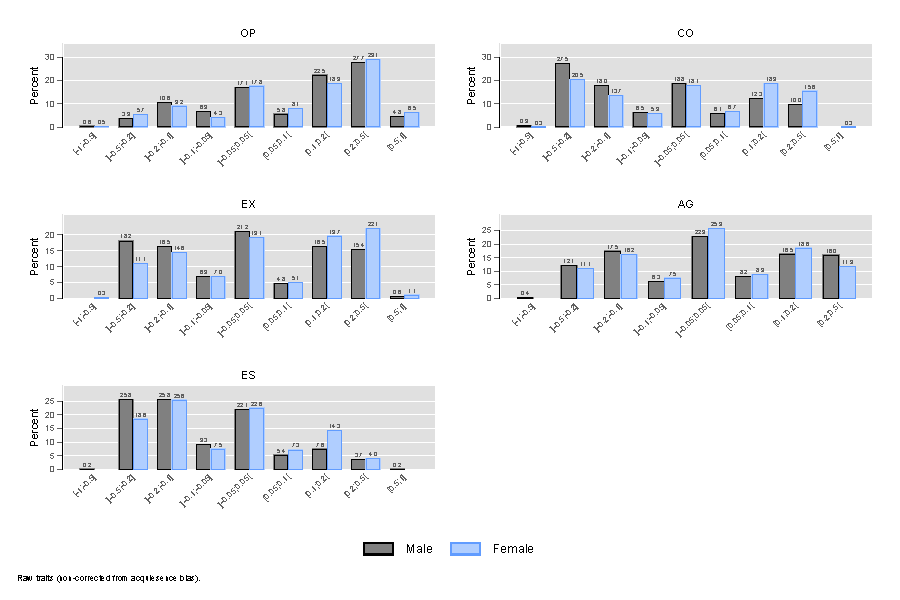
\includegraphics[scale=0.8]{INPUT/diff_gender_raw}
\caption{}
\sourcefig{NEEMSIS-1 (2016-17) \& NEEMSIS-2 (2020-21); author's calculations.}
\label{fig:diffgendercor}
\end{figure}

\begin{figure}[!h]
\raggedright
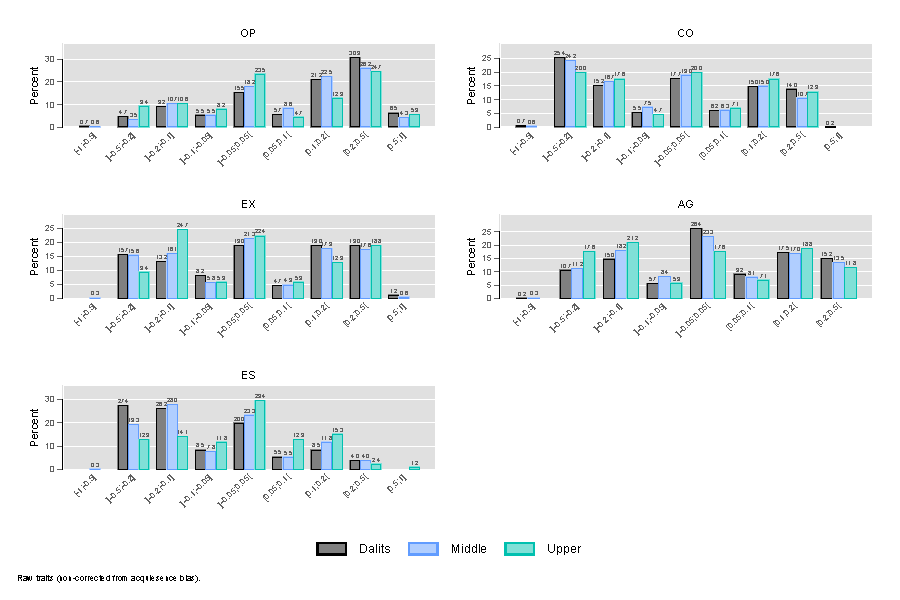
\includegraphics[scale=0.8]{INPUT/diff_caste_raw}
\caption{}
\sourcefig{NEEMSIS-1 (2016-17) \& NEEMSIS-2 (2020-21); author's calculations.}
\label{fig:diffcastecor}
\end{figure}




\clearpage
\newpage
\section{Factor analysis}

\begin{figure}[!h]
\raggedright
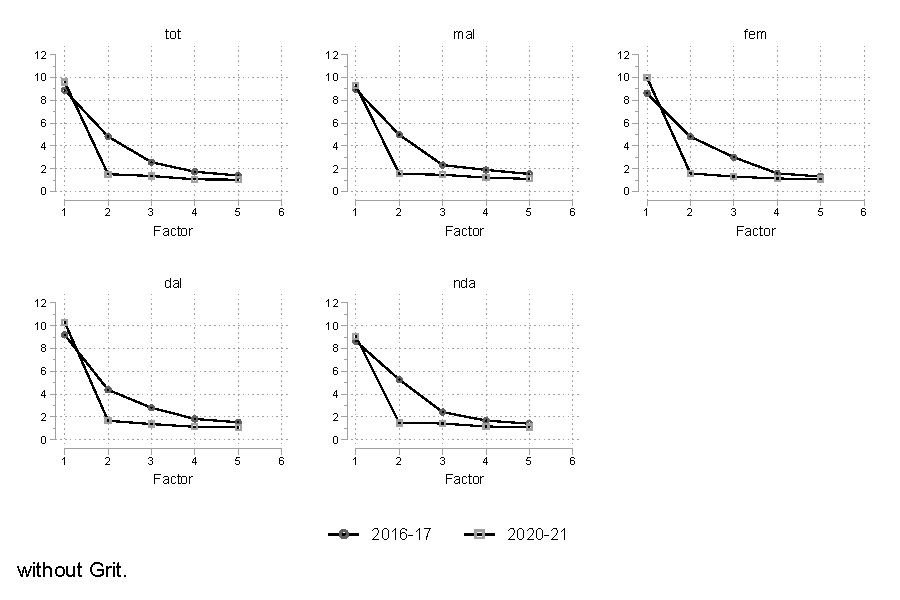
\includegraphics[scale=0.8]{INPUT/eigen_without}
\caption{}
\sourcefig{NEEMSIS-1 (2016-17) \& NEEMSIS-2 (2020-21); author's calculations.}
\label{fig:diffcastecor}
\end{figure}

\begin{figure}[!h]
\raggedright
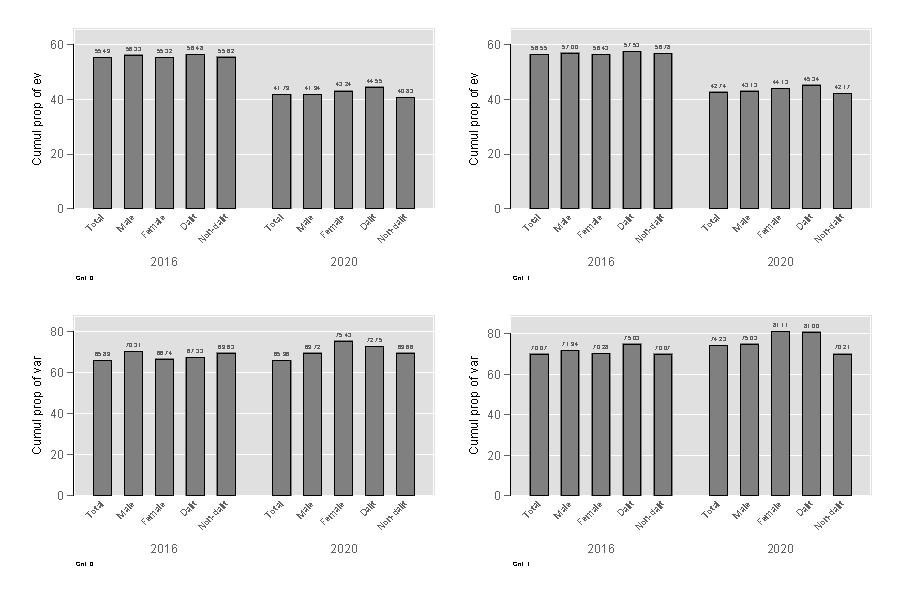
\includegraphics[scale=0.8]{INPUT/cumul}
\caption{}
\sourcefig{NEEMSIS-1 (2016-17) \& NEEMSIS-2 (2020-21); author's calculations.}
\label{fig:diffcastecor}
\end{figure}

\begin{figure}[!h]
\raggedright
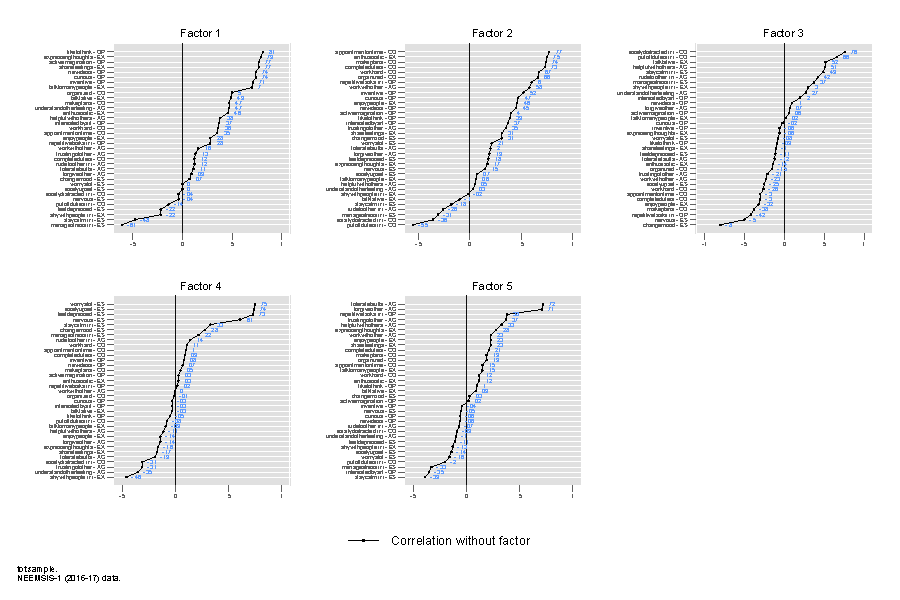
\includegraphics[scale=0.8]{INPUT/factor2016_tot_without}
\caption{}
\sourcefig{NEEMSIS-1 (2016-17); author's calculations.}
\label{fig:diffcastecor}
\end{figure}

\begin{figure}[!h]
\raggedright
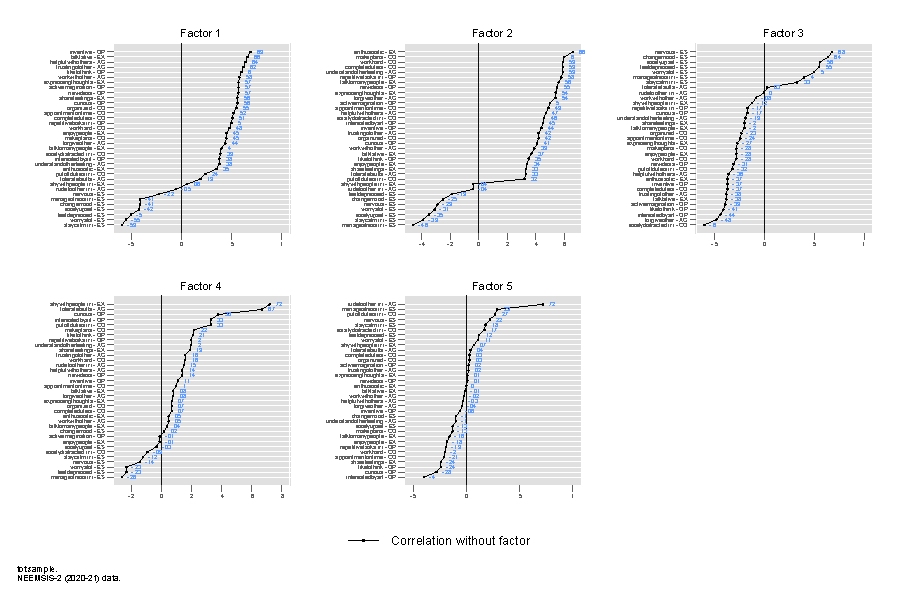
\includegraphics[scale=0.8]{INPUT/factor2020_tot_without}
\caption{}
\sourcefig{NEEMSIS-2 (2020-21); author's calculations.}
\label{fig:diffcastecor}
\end{figure}




\clearpage
\newpage
%-------------------------------------------------------------------------------%
%\begin{nolinenumbers}
\addcontentsline{toc}{section}{References}
%\bibliography{C:/Users/Arnaud/Dropbox/Arnaud/Ref_Arnaud}
\bibliography{C:/Users/Arnaud/Dropbox/Arnaud/Ref_Arnaud}
%\nocite{*}







\clearpage
\newpage
% ***********************************
\section*{Tables and figures}
\addcontentsline{toc}{section}{Tables and figures}
% ***********************************

\begin{figure}[!h]
\raggedright
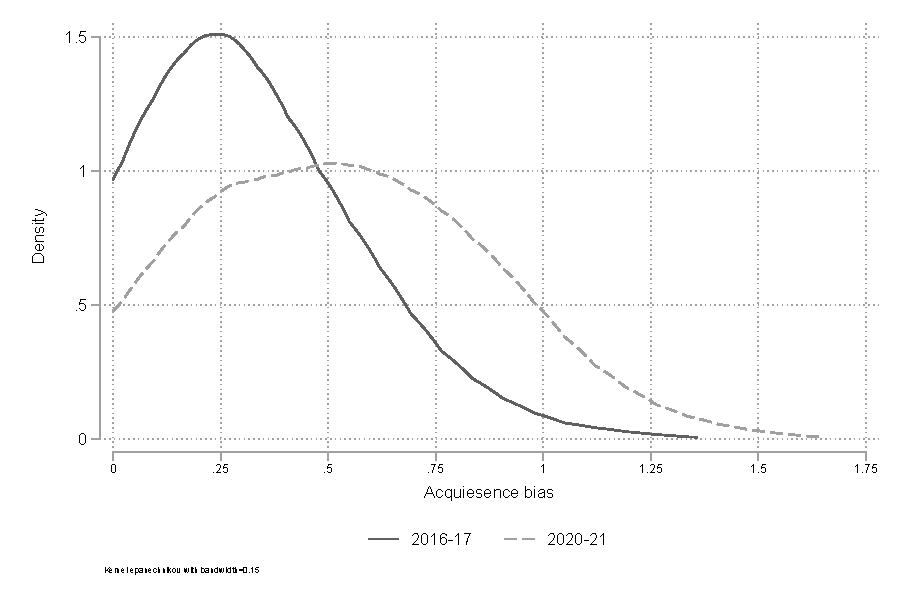
\includegraphics[scale=0.8]{INPUT/kernel_ars}
\caption{Distribution of acquiescence bias according to year -- For 953 individuals in 2016-17 and 1,316 in 2020-21 from rural Tamil Nadu, India.}
\sourcefig{NEEMSIS-1 (2016-17) \& NEEMSIS-2 (2020-21); author's calculations.}
\label{fig:ars}
\end{figure}

\begin{figure}[!h]
\raggedright
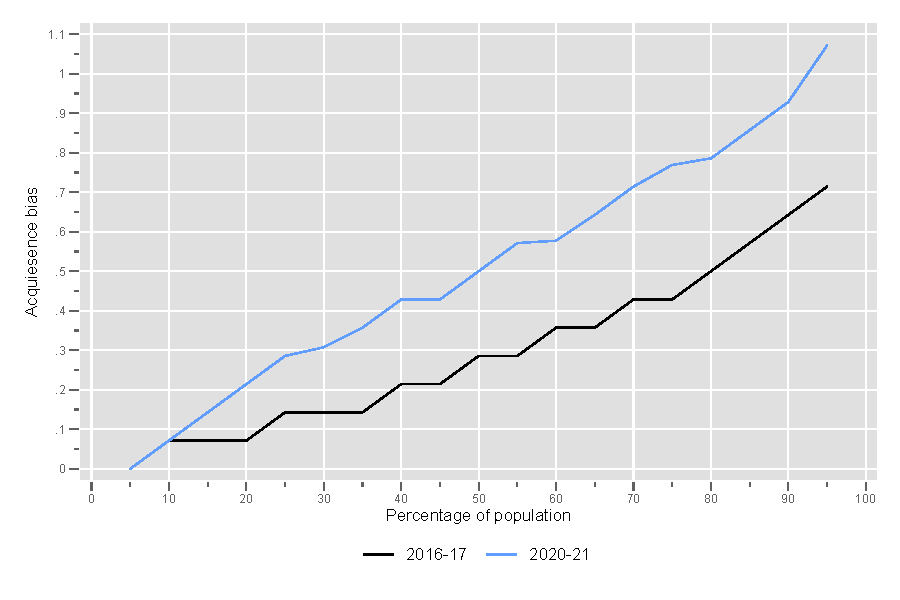
\includegraphics[scale=0.8]{INPUT/curve_ars}
\caption{Cumulative distribution of acquiescence bias -- For 953 individuals in 2016-17 and 1,316 in 2020-21 from rural Tamil Nadu, India.}
\sourcefig{NEEMSIS-1 (2016-17) \& NEEMSIS-2 (2020-21); author's calculations.}
\label{fig:curvears}
\end{figure}

\begin{figure}[!h]
\raggedright
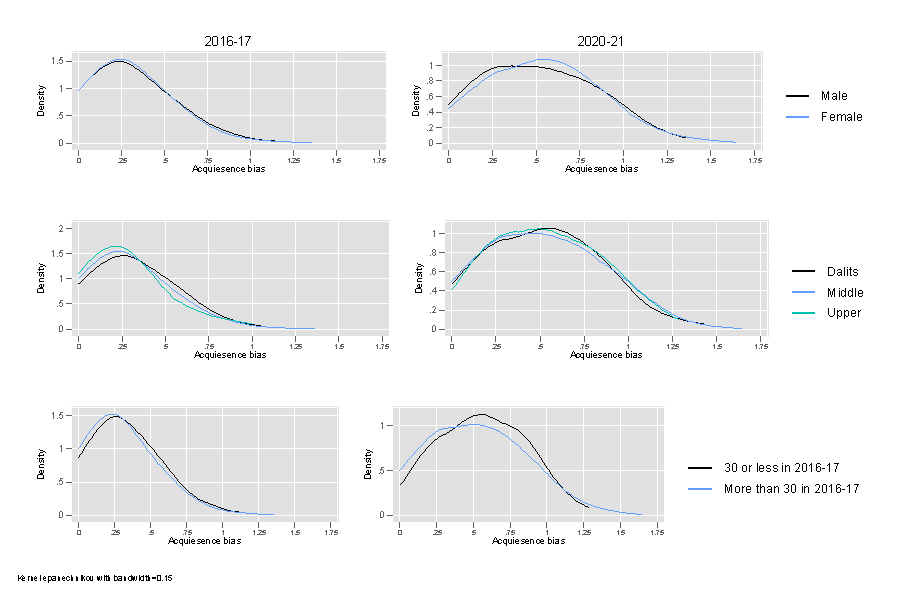
\includegraphics[scale=0.8]{INPUT/kernel_ars_sub}
\caption{Distribution of acquiescence bias according to sex, caste and gender -- For 953 individuals in 2016-17 and 1,316 in 2020-21 from rural Tamil Nadu, India.}
\sourcefig{NEEMSIS-1 (2016-17) \& NEEMSIS-2 (2020-21); author's calculations.}
\label{fig:arssub}
\end{figure}


\begin{figure}[!h]
\raggedright
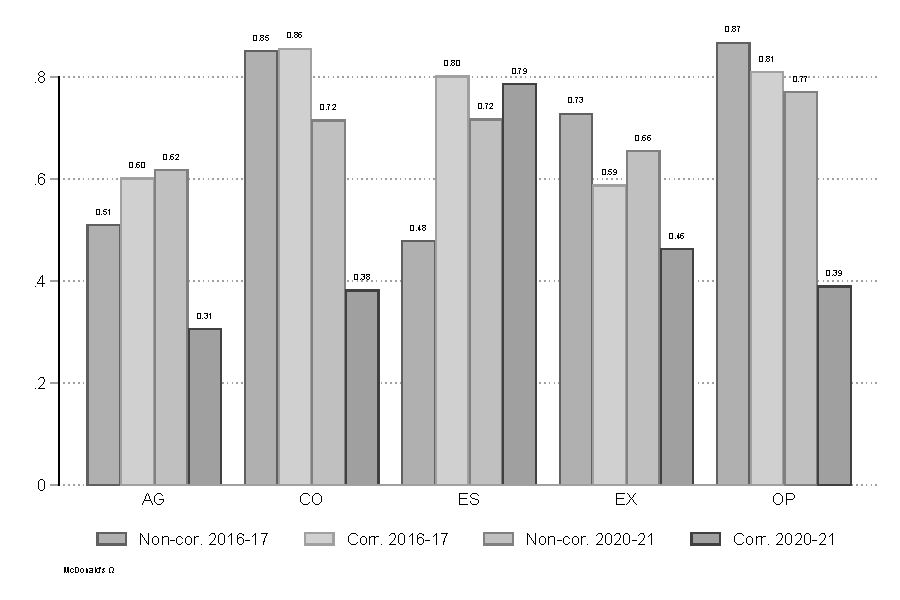
\includegraphics[scale=0.8]{INPUT/omega}
\caption{\citeauthor{McDonald1999}'s $\upomega$ -- For 953 individuals in 2016-17 and 1,316 in 2020-21 from rural Tamil Nadu, India.}
\sourcefig{NEEMSIS-1 (2016-17) \& NEEMSIS-2 (2020-21); author's calculations.}
\label{fig:omega}
\end{figure}




% \begin{figure}[!h]
% \raggedright
% 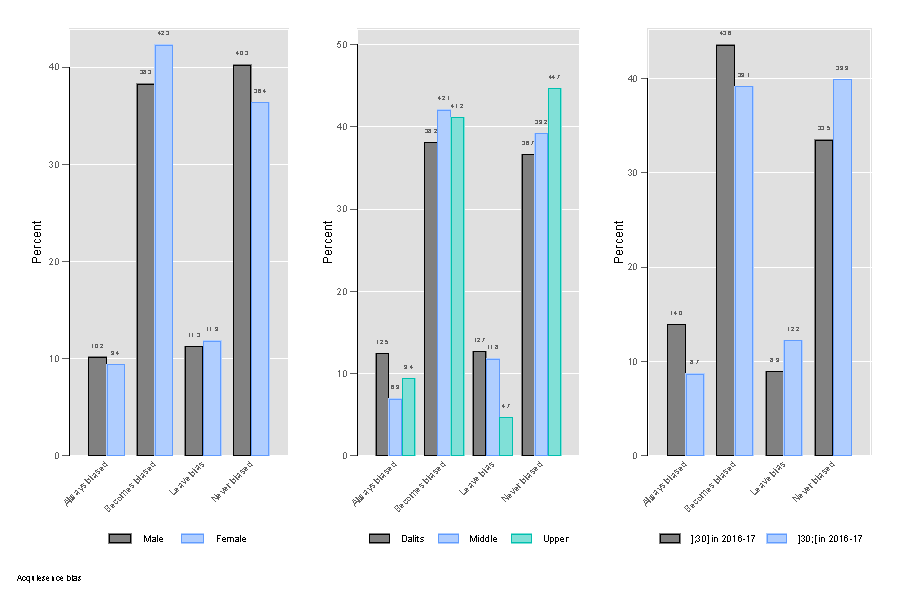
\includegraphics[scale=0.8]{INPUT/path_ars}
% \caption{Trajectory of acquiescence bias through time according to sex, caste and age -- For 835 individuals from rural Tamil Nadu, India.}
% \sourcefig{NEEMSIS-1 (2016-17) \& NEEMSIS-2 (2020-21); author's calculations.}
% \label{fig:pathars}
% \end{figure}

















\subimport{INPUT}{Big5.tex}

\begin{figure}[!h]
\raggedright
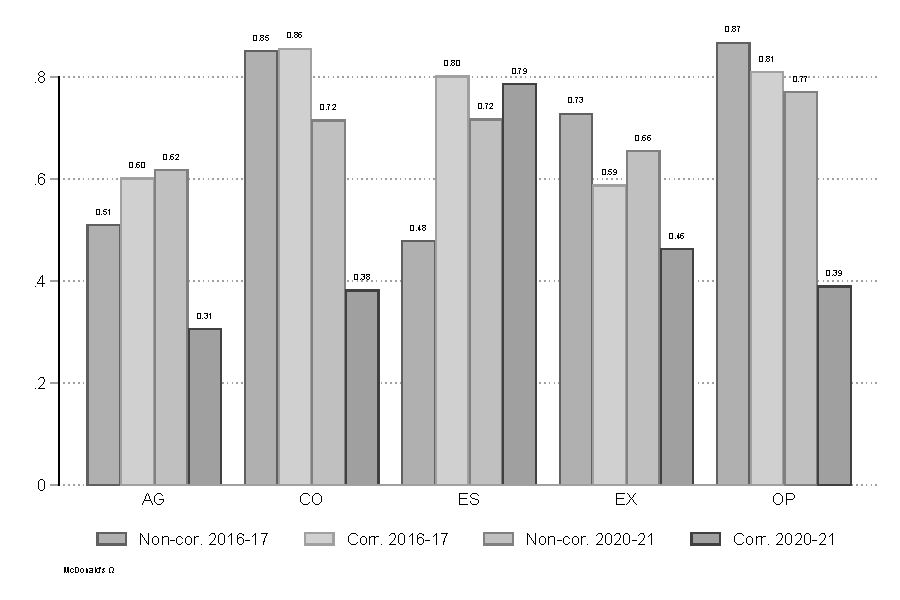
\includegraphics[scale=0.8]{INPUT/omega}
\caption{Internal consistency of Big-5 personality traits -- Distribution of \citeauthor{McDonald1999}'s $\Upomega$ through time and correction for 953 individuals in 2016-17 and 1,316 in 2020-21 from rural Tamil Nadu, India.}
\sourcefig{NEEMSIS-1 (2016-17) \& NEEMSIS-2 (2020-21); author's calculations.}
\label{fig:omega}
\end{figure}


\begin{figure}[!htb]
\raggedright
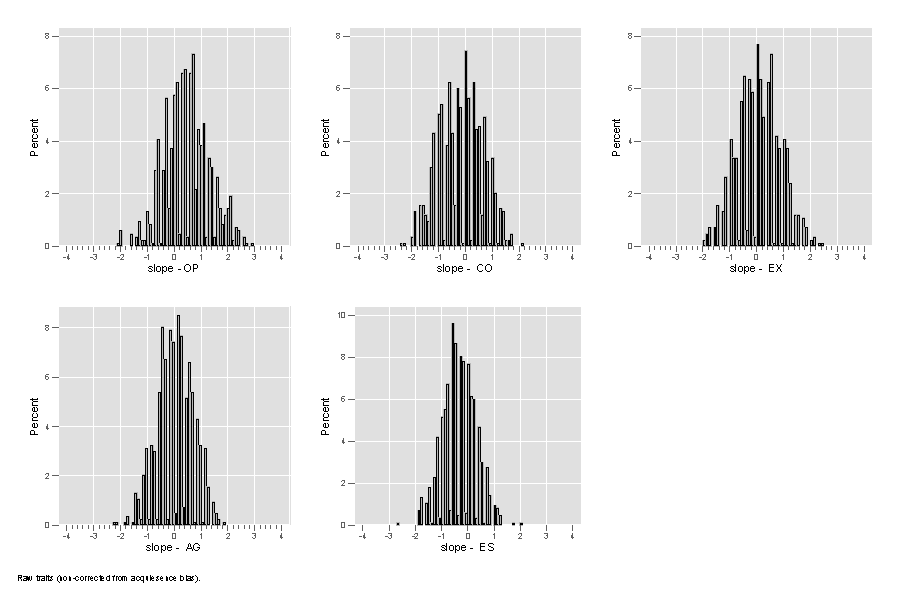
\includegraphics[scale=0.86]{INPUT/diffcont_raw}
\caption{Stability over time of Big-5 personality traits non-corrected from acquiescence bias -- Distribution of the difference of the score between 2016-17 and 2020-21 for Big-5 personality traits non-corrected from acquiescence biais for 835 individuals from rural Tamil Nadu, India.}
\sourcefig{NEEMSIS-1 (2016-17) \& NEEMSIS-2 (2020-21); author's calculations.}
\label{fig:stabraw}
\end{figure}

\begin{figure}[!htb]
\raggedright
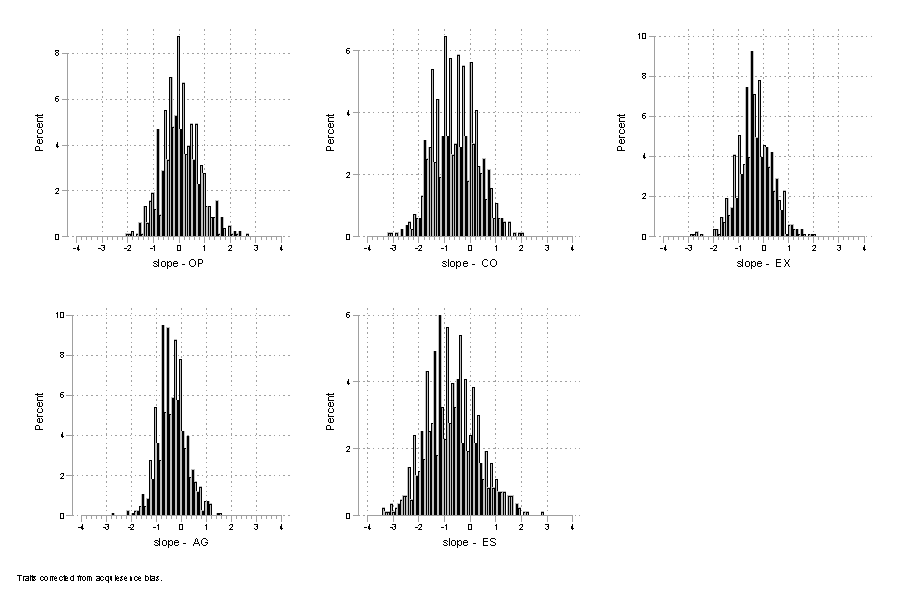
\includegraphics[scale=0.86]{INPUT/diffcont_cor}
\caption{Stability over time of Big-5 personality traits correted from acquiescence bias -- Distribution of the difference of the score between 2016-17 and 2020-21 for Big-5 personality traits corrected from acquiescence biais for 835 individuals from rural Tamil Nadu, India.}
\sourcefig{NEEMSIS-1 (2016-17) \& NEEMSIS-2 (2020-21); author's calculations.}
\label{fig:stabcor}
\end{figure}

\begin{figure}[!htb]
\raggedright
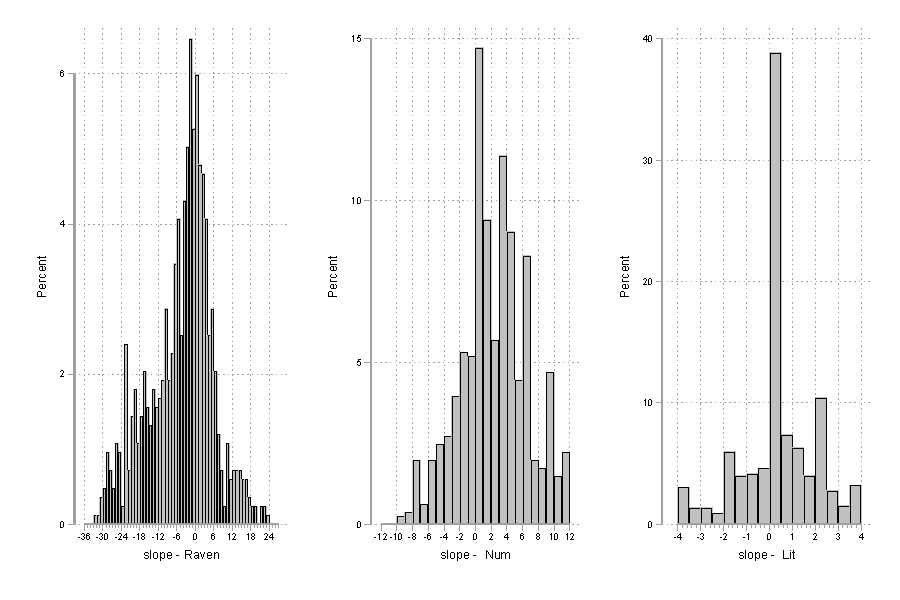
\includegraphics[scale=0.86]{INPUT/diffcont_cog}
\caption{Stability over time of cognitive skills -- Distribution of the difference of the score between 2016-17 and 2020-21 for three cognitive skills for 835 individuals from rural Tamil Nadu, India.}
\sourcefig{NEEMSIS-1 (2016-17) \& NEEMSIS-2 (2020-21); author's calculations.}
\label{fig:stabcog}
\end{figure}







\clearpage
\newpage
%-------------------------------------------------------------------------------%
\appendix
\addcontentsline{toc}{section}{Appendix}




\clearpage
\newpage
% ***********************************
\section{Factor analysis for personality traits}
\label{section:efa_big5}
% ***********************************



\clearpage
\begin{figure}[!htb]
\raggedright
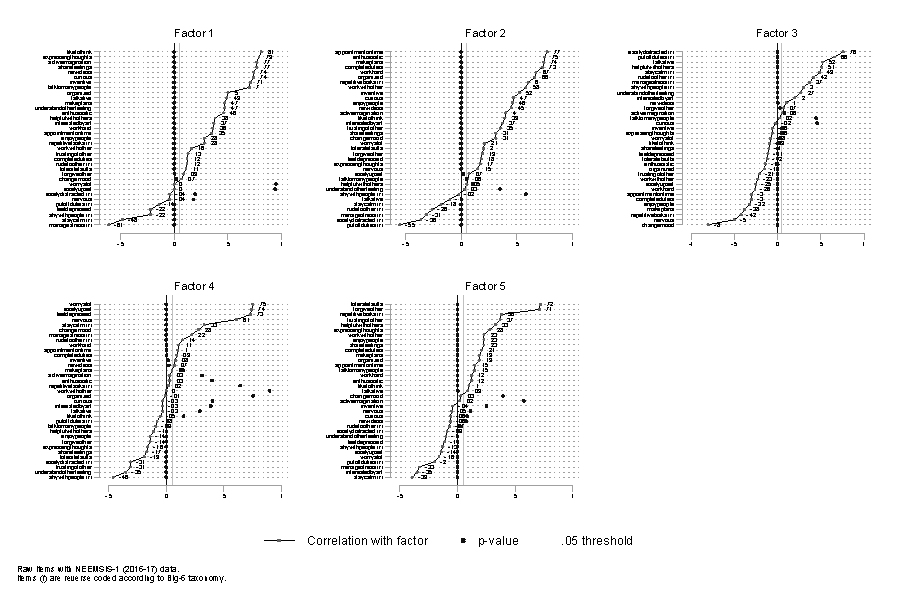
\includegraphics[width=\textwidth, angle=0]{INPUT/factor2016_2}
\caption{Results of factor analysis for 2016-17 raw items}
\sourcefig{NEEMSIS-1 (2016-17); author's calculations.}
\label{fig:resefa}
\end{figure}


\begin{figure}[!htb]
\raggedright
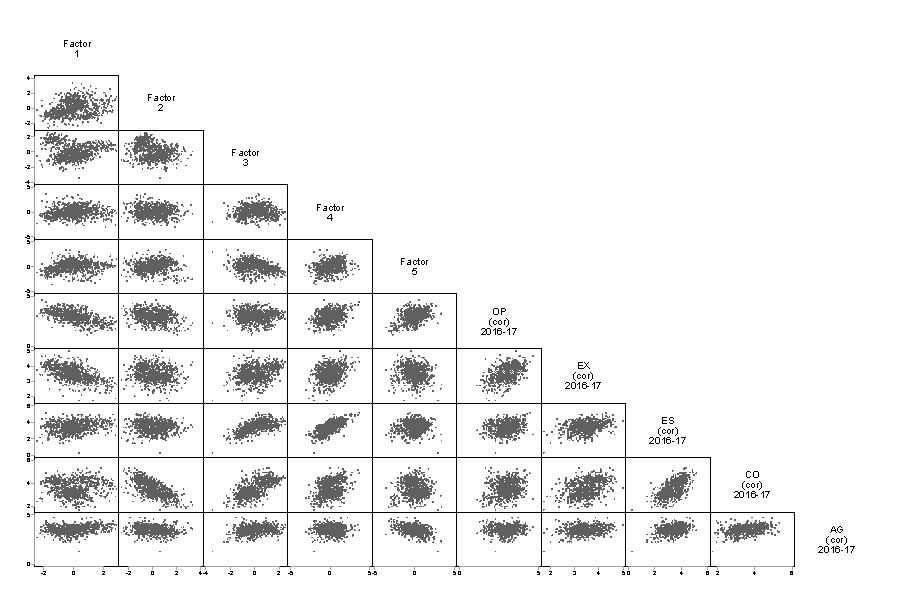
\includegraphics[scale=0.85]{INPUT/matrix_b5_efa}
\caption{Correlation between Factor from EFA and Big-5 personality traits}
\sourcefig{NEEMSIS-1 (2016-17); author's calculations.}
\label{fig:descXY}
\end{figure}




\clearpage
\newpage
%-------------------------------------------------------------------------------%
\setcounter{tocdepth}5
\tableofcontents


\end{document}